\documentclass[a4paper]{elsarticle}

\usepackage{amsmath,amssymb,amsfonts}
\usepackage{graphicx}
\usepackage{booktabs}
\usepackage{hyperref}
\usepackage{listings}
\usepackage{xcolor}
\usepackage{algorithm}
\usepackage{algpseudocode}
\usepackage{tikz}
\usetikzlibrary{arrows.meta,positioning,shapes.geometric,fit,backgrounds,calc}

\lstset{
  language=Python,
  basicstyle=\ttfamily\footnotesize,
  keywordstyle=\color{blue},
  commentstyle=\color{gray},
  stringstyle=\color{red!70!black},
  frame=single,
  breaklines=true,
  captionpos=b,
}

\journal{SoftwareX}

\begin{document}

\begin{frontmatter}

\title{\texttt{weatherisk}: A Python Package for Spatial Clustering of Climate Extremes via Max-Stable Processes}

\author[awi]{Widad Kchikach\corref{cor1}}
\ead{widad.kchikach@awi.de}
\cortext[cor1]{Corresponding author}

\affiliation[awi]{organization={Alfred Wegener Institute for Polar and Marine Research},
  city={Bremerhaven},
  country={Germany}}

\begin{abstract}
We present \texttt{weatherisk}, an open-source Python package that implements
the complete pipeline for clustering spatial climate extremes using
max-stable processes.
The package reproduces and extends an established R-based methodology
for modelling the spatial dependence structure of extreme weather events:
it simulates non-stationary max-stable processes on regular grids,
estimates local anisotropy parameters via pairwise composite likelihood,
and clusters grid cells by ellipse-shape dissimilarity to identify regions
of homogeneous extremal dependence.
Two clustering approaches are supported: a local-estimate-based method
(LEC) using ellipse-overlap dissimilarity, and an extremal-dependence-based
method (EDC) using madogram-derived extremal coefficients.
\texttt{weatherisk} consolidates a previously fragmented R/Shell workflow
into a single, tested, pip-installable Python library with a command-line
interface.
Correctness is verified by 50~automated cross-validation and R-parity
tests that compare every pipeline stage against the original R code.
We demonstrate the package on both synthetic data and 20~years of NOAA
CPC daily precipitation data, producing spatial dependence cluster maps
over a European--Middle Eastern domain.
The modular architecture supports future extensions to risk quantification,
economic exposure weighting, and forward-looking climate projections.
\end{abstract}

\begin{keyword}
spatial extremes \sep max-stable process \sep
spatial clustering \sep anisotropy \sep Python \sep
composite likelihood
\end{keyword}

\end{frontmatter}

%% ============================================================
%% CODE METADATA TABLE (required by SoftwareX)
%% ============================================================
\begin{table}[!ht]
\caption{Code metadata.}\label{tab:metadata}
\centering
\footnotesize
\begin{tabular}{@{}p{4.5cm}p{7.2cm}@{}}
\toprule
\textbf{Metadata description} & \textbf{Value} \\
\midrule
Current code version & 0.1.0 \\
Permanent link to code/repository & \url{https://github.com/xxx/weatherisk} \\
Permanent link to Reproducible Capsule & (to be added) \\
Legal Code License & MIT \\
Code versioning system used & git \\
Software code languages, tools, and services used & Python~3 \\
Compilation requirements, operating environments \& dependencies &
  Python~$\geq$3.10; NumPy~$\geq$1.24; SciPy~$\geq$1.10;
  pandas~$\geq$2.0; matplotlib~$\geq$3.7; Click~$\geq$8.0;
  xarray~$\geq$2023.1; netCDF4~$\geq$1.6;
  scikit-learn~$\geq$1.3; Cartopy~$\geq$0.21;
  h5py~$\geq$3.8 \\
If available, link to developer documentation/manual &
  \url{https://github.com/xxx/weatherisk} \\
Support email for questions & widad.kchikach@awi.de \\
\bottomrule
\end{tabular}
\end{table}

%% ============================================================
\section{Motivation and significance}
\label{sec:motivation}
%% ============================================================

Extreme climate events---heatwaves, heavy precipitation---exhibit
spatial dependence that must be modelled to understand regional
hazard patterns.
Two nearby weather stations are likely to experience a heatwave
simultaneously; characterising this dependence structure is essential
for identifying coherent risk regions~\cite{davison2012}.
Max-stable processes provide a principled framework for modelling
such spatial extremes, capturing the joint tail behaviour of a
spatial field through a small number of
parameters~\cite{dehaan2006,padoan2010}.

A key challenge is \emph{clustering}: partitioning a spatial domain
into regions of homogeneous extremal dependence, so that within each
region a single set of dependence parameters adequately describes the
tail structure.
Previous work by the authors~\cite{justus2024} developed an R-based
pipeline that
(i)~simulates non-stationary max-stable processes,
(ii)~estimates local parameters via pairwise composite likelihood,
(iii)~constructs an ellipse-shape dissimilarity matrix, and
(iv)~applies hierarchical clustering.
However, the original implementation is split across multiple R scripts
and SLURM shell orchestration files, making reproducibility and
extension difficult.

\texttt{weatherisk} addresses this gap by consolidating the entire
workflow into a single, well-tested Python package.
It provides a faithful port of the R methodology together with:
\begin{itemize}
\item extreme-value pre-processing (GEV fitting, block-maxima
  extraction, Fr\'{e}chet transform) for real climate data;
\item a real-data pipeline for NOAA CPC daily climate data
  (precipitation and temperature), producing filled-region
  Cartopy cluster maps;
\item scalable estimation and clustering strategies for global
  grids; and
\item a command-line interface with multiple pipeline flows.
\end{itemize}

The architecture is designed to support future extensions such as
per-cluster tail-risk metrics (VaR, ES), economic exposure weighting,
and scenario-based projections.

No existing Python package provides this combination of non-stationary
max-stable simulation, local composite-likelihood estimation, and
ellipse-based spatial clustering.
While \texttt{scikit-extremes} and \texttt{pyextremes} focus on
univariate extreme-value analysis, and \texttt{SpatialExtremes} (R)
implements max-stable simulation, none offer the integrated
estimation--clustering pipeline that \texttt{weatherisk} provides.

%% ============================================================
\section{Software description}
\label{sec:description}
%% ============================================================

\subsection{Software architecture}
\label{sec:architecture}

\begin{sloppypar}
\texttt{weatherisk} is organised as a pip-installable
Python package (\texttt{pyproject.toml}; PEP~621)
with 18~modules, a~CLI entry point, and 105~automated tests
(including 50~cross-validation and R-parity tests against the
original R code; see Section~\ref{sec:verification}).
\end{sloppypar}
Figure~\ref{fig:architecture} shows the package structure and data flow.

The modules are grouped into four tiers:
\begin{enumerate}
\item \textbf{Core mathematics}
  (no inter-module dependencies):
  \texttt{grid}, \texttt{covariance},
  \texttt{para\-meters}, \texttt{extremes},
  \texttt{risk}, \texttt{netcdf}, \texttt{io}.
\item \textbf{Simulation and estimation}:
  \texttt{simu\-lation}
  (depends on \texttt{grid},
  \texttt{covar\-iance}),
  \texttt{density}
  (depends on \texttt{covar\-iance}),
  \texttt{risk\_pipe\-line}
  (standalone post-processing).
\item \textbf{Clustering and smoothing}:
  \texttt{estimation}, \texttt{clustering}, \texttt{scalable}.
\item \textbf{Orchestration}:
  \texttt{plotting}, \texttt{pipeline}, \texttt{cli}.
\end{enumerate}

\begin{figure}[ht]
\centering
\resizebox{\columnwidth}{!}{%
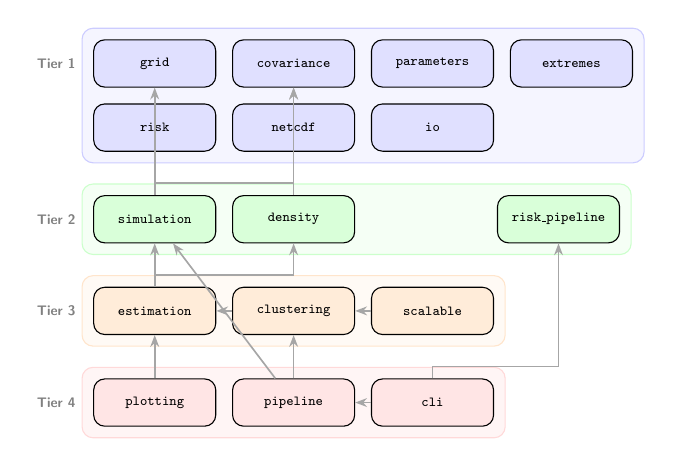
\begin{tikzpicture}[
  module/.style={draw, rounded corners, minimum width=1.55cm, minimum height=0.6cm,
    font=\ttfamily\tiny, align=center},
  tier1/.style={module, fill=blue!12},
  tier2/.style={module, fill=green!15},
  tier3/.style={module, fill=orange!15},
  tier4/.style={module, fill=red!10},
  arr/.style={-{Stealth[length=1.5mm]}, semithick, gray!70},
  tierlab/.style={font=\sffamily\tiny\bfseries, text=gray},
  node distance=0.25cm and 0.2cm,
]
% --- Tier 1: Core math, row 1 (4 modules) ---
\node[tier1] (grid)        {grid};
\node[tier1, right=of grid] (cov)    {covariance};
\node[tier1, right=of cov]  (param)  {parameters};
\node[tier1, right=of param](extr)   {extremes};
% --- Tier 1: Core math, row 2 (3 modules) ---
\node[tier1, below=0.2cm of grid]  (risk)  {risk};
\node[tier1, right=of risk]        (nc)    {netcdf};
\node[tier1, right=of nc]          (iom)   {io};

% --- Tier 2: Simulation & estimation ---
\node[tier2, below=0.55cm of risk]  (sim)  {simulation};
\node[tier2, right=of sim]          (dens) {density};
\node[tier2, right=1.8cm of dens]   (rpipe){risk\_pipeline};

% --- Tier 3: Clustering & smoothing ---
\node[tier3, below=0.55cm of sim]   (est)  {estimation};
\node[tier3, right=of est]          (clust){clustering};
\node[tier3, right=of clust]        (scal) {scalable};

% --- Tier 4: Orchestration ---
\node[tier4, below=0.55cm of est]   (plot) {plotting};
\node[tier4, right=of plot]         (pipe) {pipeline};
\node[tier4, right=of pipe]         (cli)  {cli};

% --- Dependencies (arrows) ---
\draw[arr] (sim)  -- (grid);
\draw[arr] (sim.north)  -- ++(0,0.15) -| (cov.south);
\draw[arr] (dens.north) -- ++(0,0.15) -| (cov.south);
\draw[arr] (est)  -- (sim);
\draw[arr] (est.north)  -- ++(0,0.15) -| (dens.south);
\draw[arr] (clust)-- (est);
\draw[arr] (scal) -- (clust);
\draw[arr] (pipe) -- (sim);
\draw[arr] (pipe.north) -- ++(0,0.15) -| (clust.south);
\draw[arr] (cli)  -- (pipe);
\draw[arr] (cli.north)  -- ++(0,0.15) -| (rpipe.south);
\draw[arr] (plot) -- (est);

% --- Tier labels ---
\node[tierlab, left=0.1cm of grid]   {Tier 1};
\node[tierlab, left=0.1cm of sim]    {Tier 2};
\node[tierlab, left=0.1cm of est]    {Tier 3};
\node[tierlab, left=0.1cm of plot]   {Tier 4};

% --- Background boxes ---
\begin{scope}[on background layer]
  \node[fit=(grid)(extr)(risk)(iom), fill=blue!4, draw=blue!20, rounded corners, inner sep=4pt] {};
  \node[fit=(sim)(rpipe), fill=green!4, draw=green!20, rounded corners, inner sep=4pt] {};
  \node[fit=(est)(scal), fill=orange!4, draw=orange!20, rounded corners, inner sep=4pt] {};
  \node[fit=(plot)(cli), fill=red!4, draw=red!15, rounded corners, inner sep=4pt] {};
\end{scope}
\end{tikzpicture}%
}% end resizebox
\caption{Module dependency structure of \texttt{weatherisk}.
  Tier~1 modules have no inter-package dependencies;
  higher tiers depend only on modules in the same or lower tiers.
  Arrows indicate \texttt{import} dependencies.}
\label{fig:architecture}
\end{figure}

\subsection{Software functionalities}
\label{sec:functionalities}

This section describes the key functionalities of the package.
Each subsection corresponds to a step in the clustering pipeline,
progressing from covariance modelling through simulation, estimation,
and clustering.  All functionality described here has been ported
from the original R implementation and verified against it (see
Section~\ref{sec:verification}).

\subsubsection{Covariance model (\texttt{covariance} module)}

The \texttt{covariance} module implements the stationary anisotropic
covariance function, which depends on a spatial lag vector, a
smoothness exponent, and a precision matrix encoding ellipse semi-axes
and rotation angle.  The non-stationary variant blends two local
anisotropy matrices through a harmonic mean, reducing to the
stationary case when both parameter sets are identical.

Key functions:
\begin{itemize}
\item \texttt{cov\_fkt\_2d(h, a, b, gamma, alpha)} --- stationary
  anisotropic covariance for a spatial lag \texttt{h};
\item \texttt{cov\_fkt\_2d\_nonstat2(h, a1, b1, g1, a2, b2, g2,
  alpha)} --- non-stationary variant blending two parameter sets;
\item \texttt{cov\_to\_ec(rho, df)} --- converts correlation to
  extremal coefficient via the extremal-$t$ model;
\item \texttt{ec\_to\_cov(theta, df)} --- numerically inverts the
  extremal coefficient back to correlation.
\end{itemize}

\subsubsection{Max-stable process simulation (\texttt{simulation} module)}

The \texttt{simulation} module generates realisations of a
max-stable process following the spectral
representation of~\cite{schlather2002}.
A Poisson point process generates arrival times; for each arrival a
Gaussian spectral function is drawn from a multivariate normal with
covariance matrix obtained via Cholesky decomposition.
The pointwise maximum over all spectral functions, scaled by the
Poisson arrival, yields the max-stable realisation with Student-$t$
margins, which are normalised to unit Fr\'{e}chet.

Key function:
\begin{itemize}
\item \texttt{simulate\_non\_stat(params, grid, n\_sim, df, alpha,
  seed)} --- simulates \texttt{n\_sim} realisations on a given grid
  with spatially varying anisotropy.
\end{itemize}

\subsubsection{Pairwise composite likelihood estimation (\texttt{density} and \texttt{estimation} modules)}

Local anisotropy parameters (semi-axis lengths $a$, $b$ and rotation
angle $\gamma$) at each grid cell are estimated by maximising a
pairwise composite log-likelihood~\cite{padoan2010} over all pairs
within a spatial neighbourhood.  Optimisation uses Latin Hypercube
initialisation followed by L-BFGS-B~\cite{byrd1995}.

The \texttt{density} module provides the bivariate density and its
derivatives; the \texttt{estimation} module orchestrates the local
and in-cluster estimation.

Key functions:
\begin{itemize}
\item \texttt{pairwise\_density\_optim\_local(data, grid, ...)} ---
  local parameter estimation at a single grid cell;
\item \texttt{calc\_local\_estimates(data, grid, ...)} ---
  estimates parameters at all grid cells, with optional parallel
  execution;
\item \texttt{smooth\_estimates(raw\_est, grid, sigma)} ---
  spatial Gaussian smoothing of the raw local estimates (with circular
  wrapping for the rotation angle);
\item \texttt{calc\_estimates\_in\_clusters(data, clusters, ...)} ---
  re-estimates parameters within each cluster using all data from
  the cluster's grid cells.
\end{itemize}

\subsubsection{Clustering (\texttt{clustering} module)}

Two clustering methods are implemented:

\begin{enumerate}
\item \textbf{LEC --- Local Estimate Clustering (ellipse dissimilarity)}:
  For each pair of grid cells, the Jaccard-like overlap between
  estimated anisotropy ellipses is computed and scaled to a
  dissimilarity in $[0, 100]$.  Hierarchical agglomerative clustering
  (average linkage) is applied, and $k$ is determined by a threshold
  on merge heights.

\item \textbf{EDC --- Extremal Dependence Clustering (Saunders method)}:
  Rank-based madogram estimation of pairwise extremal coefficients
  yields an alternative dissimilarity
  matrix~\cite{saunders2021,cooley2006}.  The same hierarchical
  clustering procedure is applied.
\end{enumerate}

Key functions:
\begin{itemize}
\item \texttt{ellipse\_dissimilarity(est, grid)} --- computes the
  full pairwise dissimilarity matrix from smoothed estimates;
\item \texttt{saunders\_clustering(data, grid, ...)} --- end-to-end
  EDC clustering using the madogram;
\item \texttt{cluster\_from\_dissimilarity(D, quantile\_threshold)} ---
  applies hierarchical clustering with automatic $k$ selection.
\end{itemize}

\subsubsection{Extreme-value pre-processing (\texttt{extremes} module)}

For real climate data, the marginal distributions must be standardised
before dependence modelling.
The \texttt{extremes} module fits GEV distributions to annual block
maxima and transforms them to unit Fr\'{e}chet margins, which is
the standard marginal assumption for max-stable process modelling.

Key functions:
\begin{itemize}
\item \texttt{fit\_gev(data)} --- maximum-likelihood estimation of
  GEV parameters (location, scale, shape);
\item \texttt{to\_frechet(data, gev\_params)} --- probability
  integral transform to unit Fr\'{e}chet margins.
\end{itemize}

\subsubsection{Scalable clustering for global grids (\texttt{scalable} module)}

For grids exceeding $\sim$16\,000 cells, the full dissimilarity matrix
is prohibitively large.  \texttt{weatherisk} provides a coarse-grid
proxy strategy, illustrated in Figure~\ref{fig:scalable}: local
estimation runs at full resolution (embarrassingly parallel),
clustering operates on a downsampled grid that fits in memory, and
labels are propagated back and refined at full resolution.

\begin{figure}[ht]
\centering
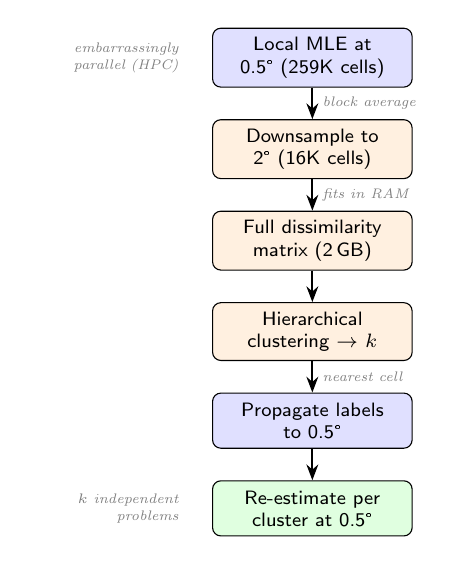
\begin{tikzpicture}[
  box/.style={draw, rounded corners=3pt, minimum width=2.4cm, minimum height=0.7cm,
    font=\sffamily\scriptsize, align=center, text width=2.3cm},
  fine/.style={box, fill=blue!12},
  coarse/.style={box, fill=orange!12},
  result/.style={box, fill=green!12},
  arr/.style={-{Stealth[length=2mm]}, thick},
  note/.style={font=\itshape\tiny, text=gray},
  node distance=0.4cm,
]

\node[fine]   (est)   {Local MLE at\\0.5\textdegree\ (259K cells)};
\node[coarse, below=of est] (down) {Downsample to\\2\textdegree\ (16K cells)};
\node[coarse, below=of down] (dmat) {Full dissimilarity\\matrix (2\,GB)};
\node[coarse, below=of dmat] (hclust) {Hierarchical\\clustering $\to$ $k$};
\node[fine,   below=of hclust] (prop) {Propagate labels\\to 0.5\textdegree};
\node[result, below=of prop] (reest) {Re-estimate per\\cluster at 0.5\textdegree};

\draw[arr] (est) -- (down) node[midway, right, note] {block average};
\draw[arr] (down) -- (dmat) node[midway, right, note] {fits in RAM};
\draw[arr] (dmat) -- (hclust);
\draw[arr] (hclust) -- (prop) node[midway, right, note] {nearest cell};
\draw[arr] (prop) -- (reest);

% HPC annotation
\node[note, left=0.3cm of est, text width=1.8cm, align=right]
  {embarrassingly\\parallel (HPC)};
\node[note, left=0.3cm of reest, text width=1.8cm, align=right]
  {$k$ independent\\problems};

\end{tikzpicture}
\caption{Coarse-grid proxy strategy for scalable clustering.
  Local estimation is embarrassingly parallel at full resolution;
  clustering operates on a downsampled grid that fits in memory;
  labels are propagated back and refined.}
\label{fig:scalable}
\end{figure}

Intermediate results are checkpointed via \texttt{save\_chunk}/\texttt{load\_chunk},
enabling SLURM job-array parallelism on HPC systems.

\subsection{Pipeline flows}
\label{sec:flows}

The CLI exposes multiple pipeline flows, illustrated in
Figure~\ref{fig:flows}.

\begin{figure*}[ht]
\centering
\resizebox{\textwidth}{!}{%
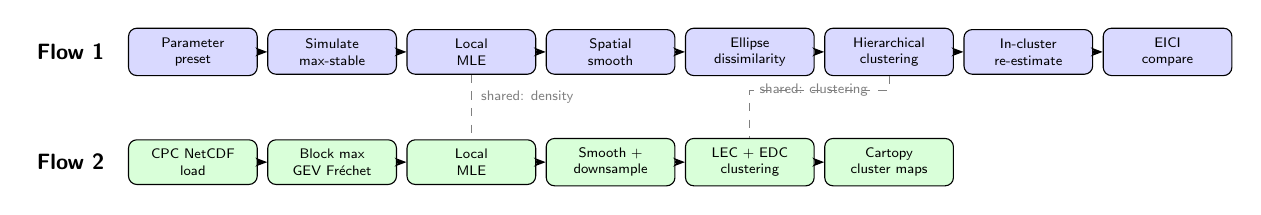
\begin{tikzpicture}[
  stepbox/.style={draw, rounded corners=3pt, minimum width=1.5cm, minimum height=0.55cm,
    font=\sffamily\tiny, align=center, text width=1.4cm},
  flow1/.style={stepbox, fill=blue!15},
  flow2/.style={stepbox, fill=green!15},
  arr/.style={-{Stealth[length=1.5mm]}, semithick},
  flowlabel/.style={font=\sffamily\footnotesize\bfseries, anchor=east},
  node distance=0.12cm and 0.12cm,
]

% ===== FLOW 1: Validation =====
\node[flowlabel] at (-0.5, 0) {Flow 1};
\node[flow1] (f1a) at (0.5,0) {Parameter\\preset};
\node[flow1, right=of f1a] (f1b) {Simulate\\max-stable};
\node[flow1, right=of f1b] (f1c) {Local\\MLE};
\node[flow1, right=of f1c] (f1d) {Spatial\\smooth};
\node[flow1, right=of f1d] (f1e) {Ellipse\\dissimilarity};
\node[flow1, right=of f1e] (f1f) {Hierarchical\\clustering};
\node[flow1, right=of f1f] (f1g) {In-cluster\\re-estimate};
\node[flow1, right=of f1g] (f1h) {EICI\\compare};

\draw[arr] (f1a) -- (f1b);
\draw[arr] (f1b) -- (f1c);
\draw[arr] (f1c) -- (f1d);
\draw[arr] (f1d) -- (f1e);
\draw[arr] (f1e) -- (f1f);
\draw[arr] (f1f) -- (f1g);
\draw[arr] (f1g) -- (f1h);

% ===== FLOW 2: CPC Maps =====
\node[flowlabel] at (-0.5, -1.4) {Flow 2};
\node[flow2] (f2a) at (0.5,-1.4) {CPC NetCDF\\load};
\node[flow2, right=of f2a] (f2b) {Block max\\GEV Fr\'{e}chet};
\node[flow2, right=of f2b] (f2c) {Local\\MLE};
\node[flow2, right=of f2c] (f2d) {Smooth +\\downsample};
\node[flow2, right=of f2d] (f2e) {LEC + EDC\\clustering};
\node[flow2, right=of f2e] (f2f) {Cartopy\\cluster maps};

\draw[arr] (f2a) -- (f2b);
\draw[arr] (f2b) -- (f2c);
\draw[arr] (f2c) -- (f2d);
\draw[arr] (f2d) -- (f2e);
\draw[arr] (f2e) -- (f2f);

% ===== Shared modules annotation =====
\draw[dashed, gray] (f1c.south) -- ++(0,-0.28) -| (f2c.north)
  node[midway, right, font=\sffamily\tiny, text=gray] {shared: density};
\draw[dashed, gray] (f1f.south) -- ++(0,-0.18) -| (f2e.north)
  node[midway, right, font=\sffamily\tiny, text=gray] {shared: clustering};

\end{tikzpicture}%
}% end resizebox
\caption{The two main pipeline flows of \texttt{weatherisk}.
  Flow~1 validates the clustering method on synthetic data.
  Flow~2 applies the method to real NOAA CPC climate observations
  and generates filled-region Cartopy cluster maps.
  Dashed lines indicate shared modules between flows.}
\label{fig:flows}
\end{figure*}

\paragraph{Flow~1: Method validation (\texttt{weatherisk validate}).}
Reproduces the clustering method on synthetic data:
parameters $\to$ simulate $\to$ local estimation $\to$ smooth $\to$
ellipse dissimilarity $\to$ hierarchical clustering $\to$ in-cluster
re-estimation.
Grid sizes of 10--51 points per axis run in minutes on a laptop.

\begin{lstlisting}[caption={Running the validation flow.},label=lst:validate]
$ weatherisk validate --params stripes \
    --resolution 10 --n-sim 20 \
    --seed 42
\end{lstlisting}

\paragraph{Flow~2: CPC cluster maps (\texttt{weatherisk maps}).}
The primary pipeline for reproducible analysis of NOAA CPC daily climate
data.  Loads 20~years of NetCDF files, computes annual block maxima,
fits GEV marginals, transforms to unit Fr\'{e}chet, performs local MLE of
anisotropy parameters $(a, b, \gamma)$, runs both LEC and EDC clustering,
and outputs filled-region Cartopy cluster maps.

\begin{lstlisting}[caption={Running the CPC maps pipeline.},label=lst:maps]
$ weatherisk maps --variable precip
\end{lstlisting}

The pipeline architecture is extensible: future versions will add
per-cluster tail-risk metrics (VaR, ES) and optional GDP~exposure
weighting for economic risk assessment.

%% ============================================================
\section{Illustrative examples}
\label{sec:examples}
%% ============================================================

\subsection{Synthetic validation}

We demonstrate Flow~1 on the ``stripes'' parameter preset, where the
semi-major axis~$b$ varies linearly with the $x$-coordinate, creating
stripe-like anisotropy regions that the clustering method should recover.

\begin{lstlisting}[caption={Python API usage for synthetic validation.},label=lst:api]
from weatherisk.parameters import get_preset
from weatherisk.pipeline import run_pipeline
from weatherisk.plotting import plot_cluster_map

p = get_preset("stripes")
result = run_pipeline(
    resolution=10, n_sim=20,
    df=p.df, alpha=p.alpha, seed=42,
)
fig = plot_cluster_map(
    result["clusters"], result["grid"]
)
fig.savefig("clusters.pdf")
\end{lstlisting}

The pipeline produces cluster assignments that align with the known
ground-truth anisotropy boundaries.
On a standard laptop (Apple M2, 16\,GB RAM), the 10$\times$10 grid
with 20~simulations completes in under 10~seconds.

Figure~\ref{fig:clustering-comparison} illustrates the two clustering
approaches.

\begin{figure}[ht]
\centering
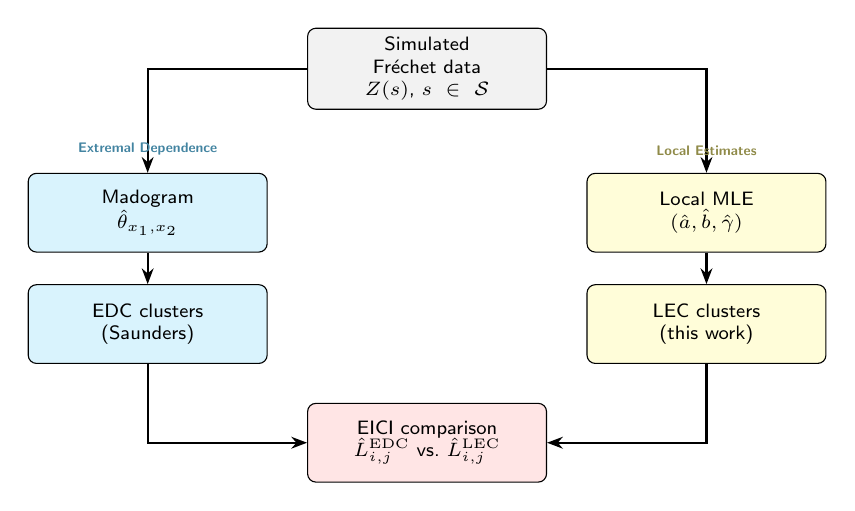
\begin{tikzpicture}[
  box/.style={draw, rounded corners=3pt, minimum width=3.0cm, minimum height=1.0cm,
    font=\sffamily\scriptsize, align=center, text width=2.8cm},
  input/.style={box, fill=gray!10},
  edc/.style={box, fill=cyan!15},
  lec/.style={box, fill=yellow!15},
  compare/.style={box, fill=red!10},
  arr/.style={-{Stealth[length=2mm]}, thick},
  node distance=0.4cm and 0.8cm,
]

% Input
\node[input] (sim) {Simulated\\Fr\'{e}chet data\\$Z(s)$, $s \in \mathcal{S}$};

% EDC branch (left)
\node[edc, below left=0.8cm and 0.5cm of sim] (mad) {Madogram\\$\hat{\theta}_{x_1,x_2}$};
\node[edc, below=of mad] (edc_clust) {EDC clusters\\(Saunders)};

% LEC branch (right)
\node[lec, below right=0.8cm and 0.5cm of sim] (mle) {Local MLE\\$(\hat{a}, \hat{b}, \hat{\gamma})$};
\node[lec, below=of mle] (lec_clust) {LEC clusters\\(this work)};

% Comparison
\node[compare, below=1.0cm of $(edc_clust)!0.5!(lec_clust)$] (eici)
  {EICI comparison\\$\hat{L}^{\mathrm{EDC}}_{i,j}$ vs.\ $\hat{L}^{\mathrm{LEC}}_{i,j}$};

% Arrows
\draw[arr] (sim) -| (mad);
\draw[arr] (sim) -| (mle);
\draw[arr] (mad) -- (edc_clust);
\draw[arr] (mle) -- (lec_clust);
\draw[arr] (edc_clust) |- (eici);
\draw[arr] (lec_clust) |- (eici);

% Labels
\node[font=\sffamily\tiny\bfseries, text=cyan!60!black, above=0.1cm of mad]
  {Extremal Dependence};
\node[font=\sffamily\tiny\bfseries, text=yellow!50!black, above=0.1cm of mle]
  {Local Estimates};

\end{tikzpicture}
\caption{Comparison of the two clustering approaches.
  EDC (left) uses madogram-based extremal coefficients;
  LEC (right, this work) uses locally estimated ellipse parameters.
  The EICI metric compares goodness of fit on cluster intersections,
  following~\cite{justus2024}.}
\label{fig:clustering-comparison}
\end{figure}

\subsection{Real-data application: CPC precipitation}
\label{sec:real-data}

Flow~2 is applied to 20~years (2000--2019) of NOAA CPC daily
precipitation data over a European--Middle Eastern sub-region
(30\textdegree--65\textdegree N, 5\textdegree--55\textdegree E),
coarsened to $\sim$2\textdegree\ resolution (384~valid land cells).
Annual block maxima are computed, GEV marginals fitted, and values
transformed to unit Fr\'{e}chet margins.  Local pairwise composite
likelihood estimation yields anisotropy parameters $(a, b, \gamma)$
at each cell, which are spatially smoothed and used for both LEC
(ellipse-overlap dissimilarity) and EDC (madogram dissimilarity)
clustering with a 30\%-quantile threshold on the pairwise dissimilarity
matrix.

The LEC method identifies $k = 26$ clusters and the EDC method
identifies $k = 18$ clusters.  Figure~\ref{fig:cpc-lec-clusters}
shows the LEC clusters in detail.

\begin{figure}[ht]
\centering
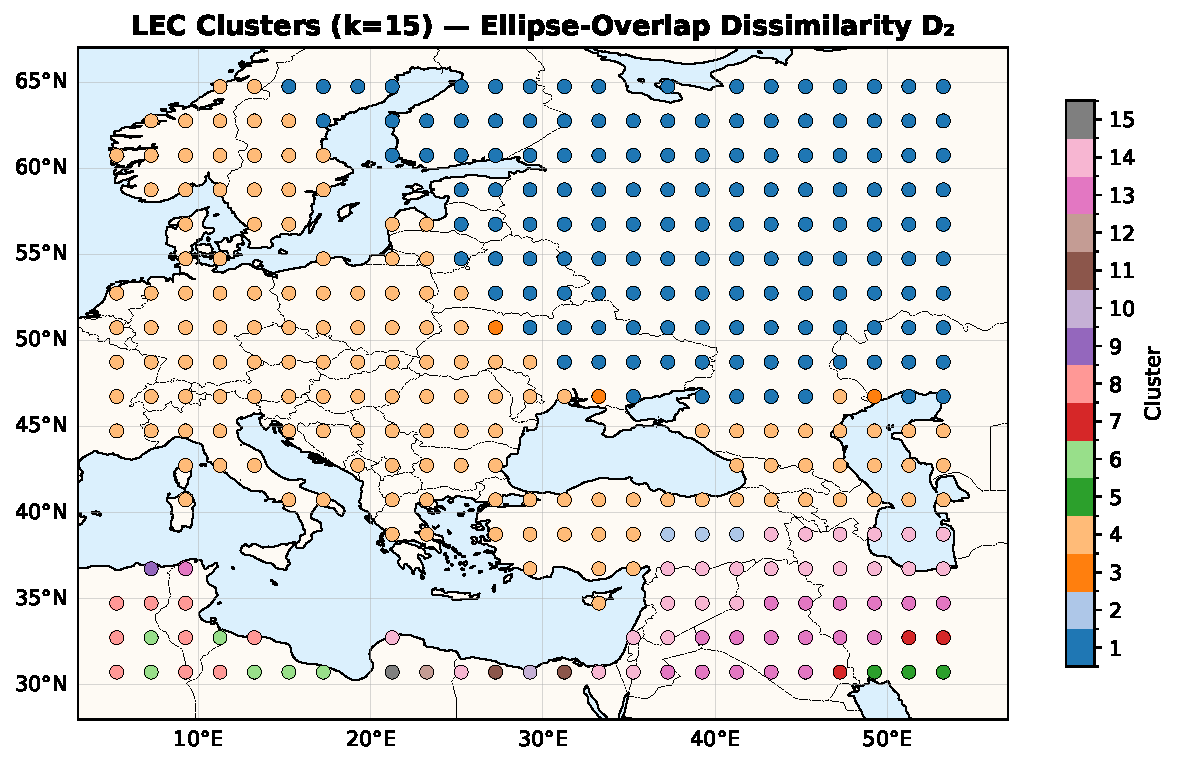
\includegraphics[width=0.95\textwidth]{figures/lec_clusters_map.pdf}
\caption{LEC spatial dependence clusters for CPC precipitation extremes
  (2000--2019, $k = 26$).  Clusters are determined by the ellipse-overlap
  dissimilarity with a 30\%-quantile threshold.  Each colour
  identifies a region of homogeneous extremal dependence structure.
  The clustering captures known climatic boundaries: the Mediterranean
  basin, Atlantic-influenced Western Europe, and continental interiors
  form distinct regions.}
\label{fig:cpc-lec-clusters}
\end{figure}

Figure~\ref{fig:cpc-summary} shows a summary panel including both
LEC and EDC cluster maps alongside the estimated anisotropy parameters.

\begin{figure*}[ht]
\centering
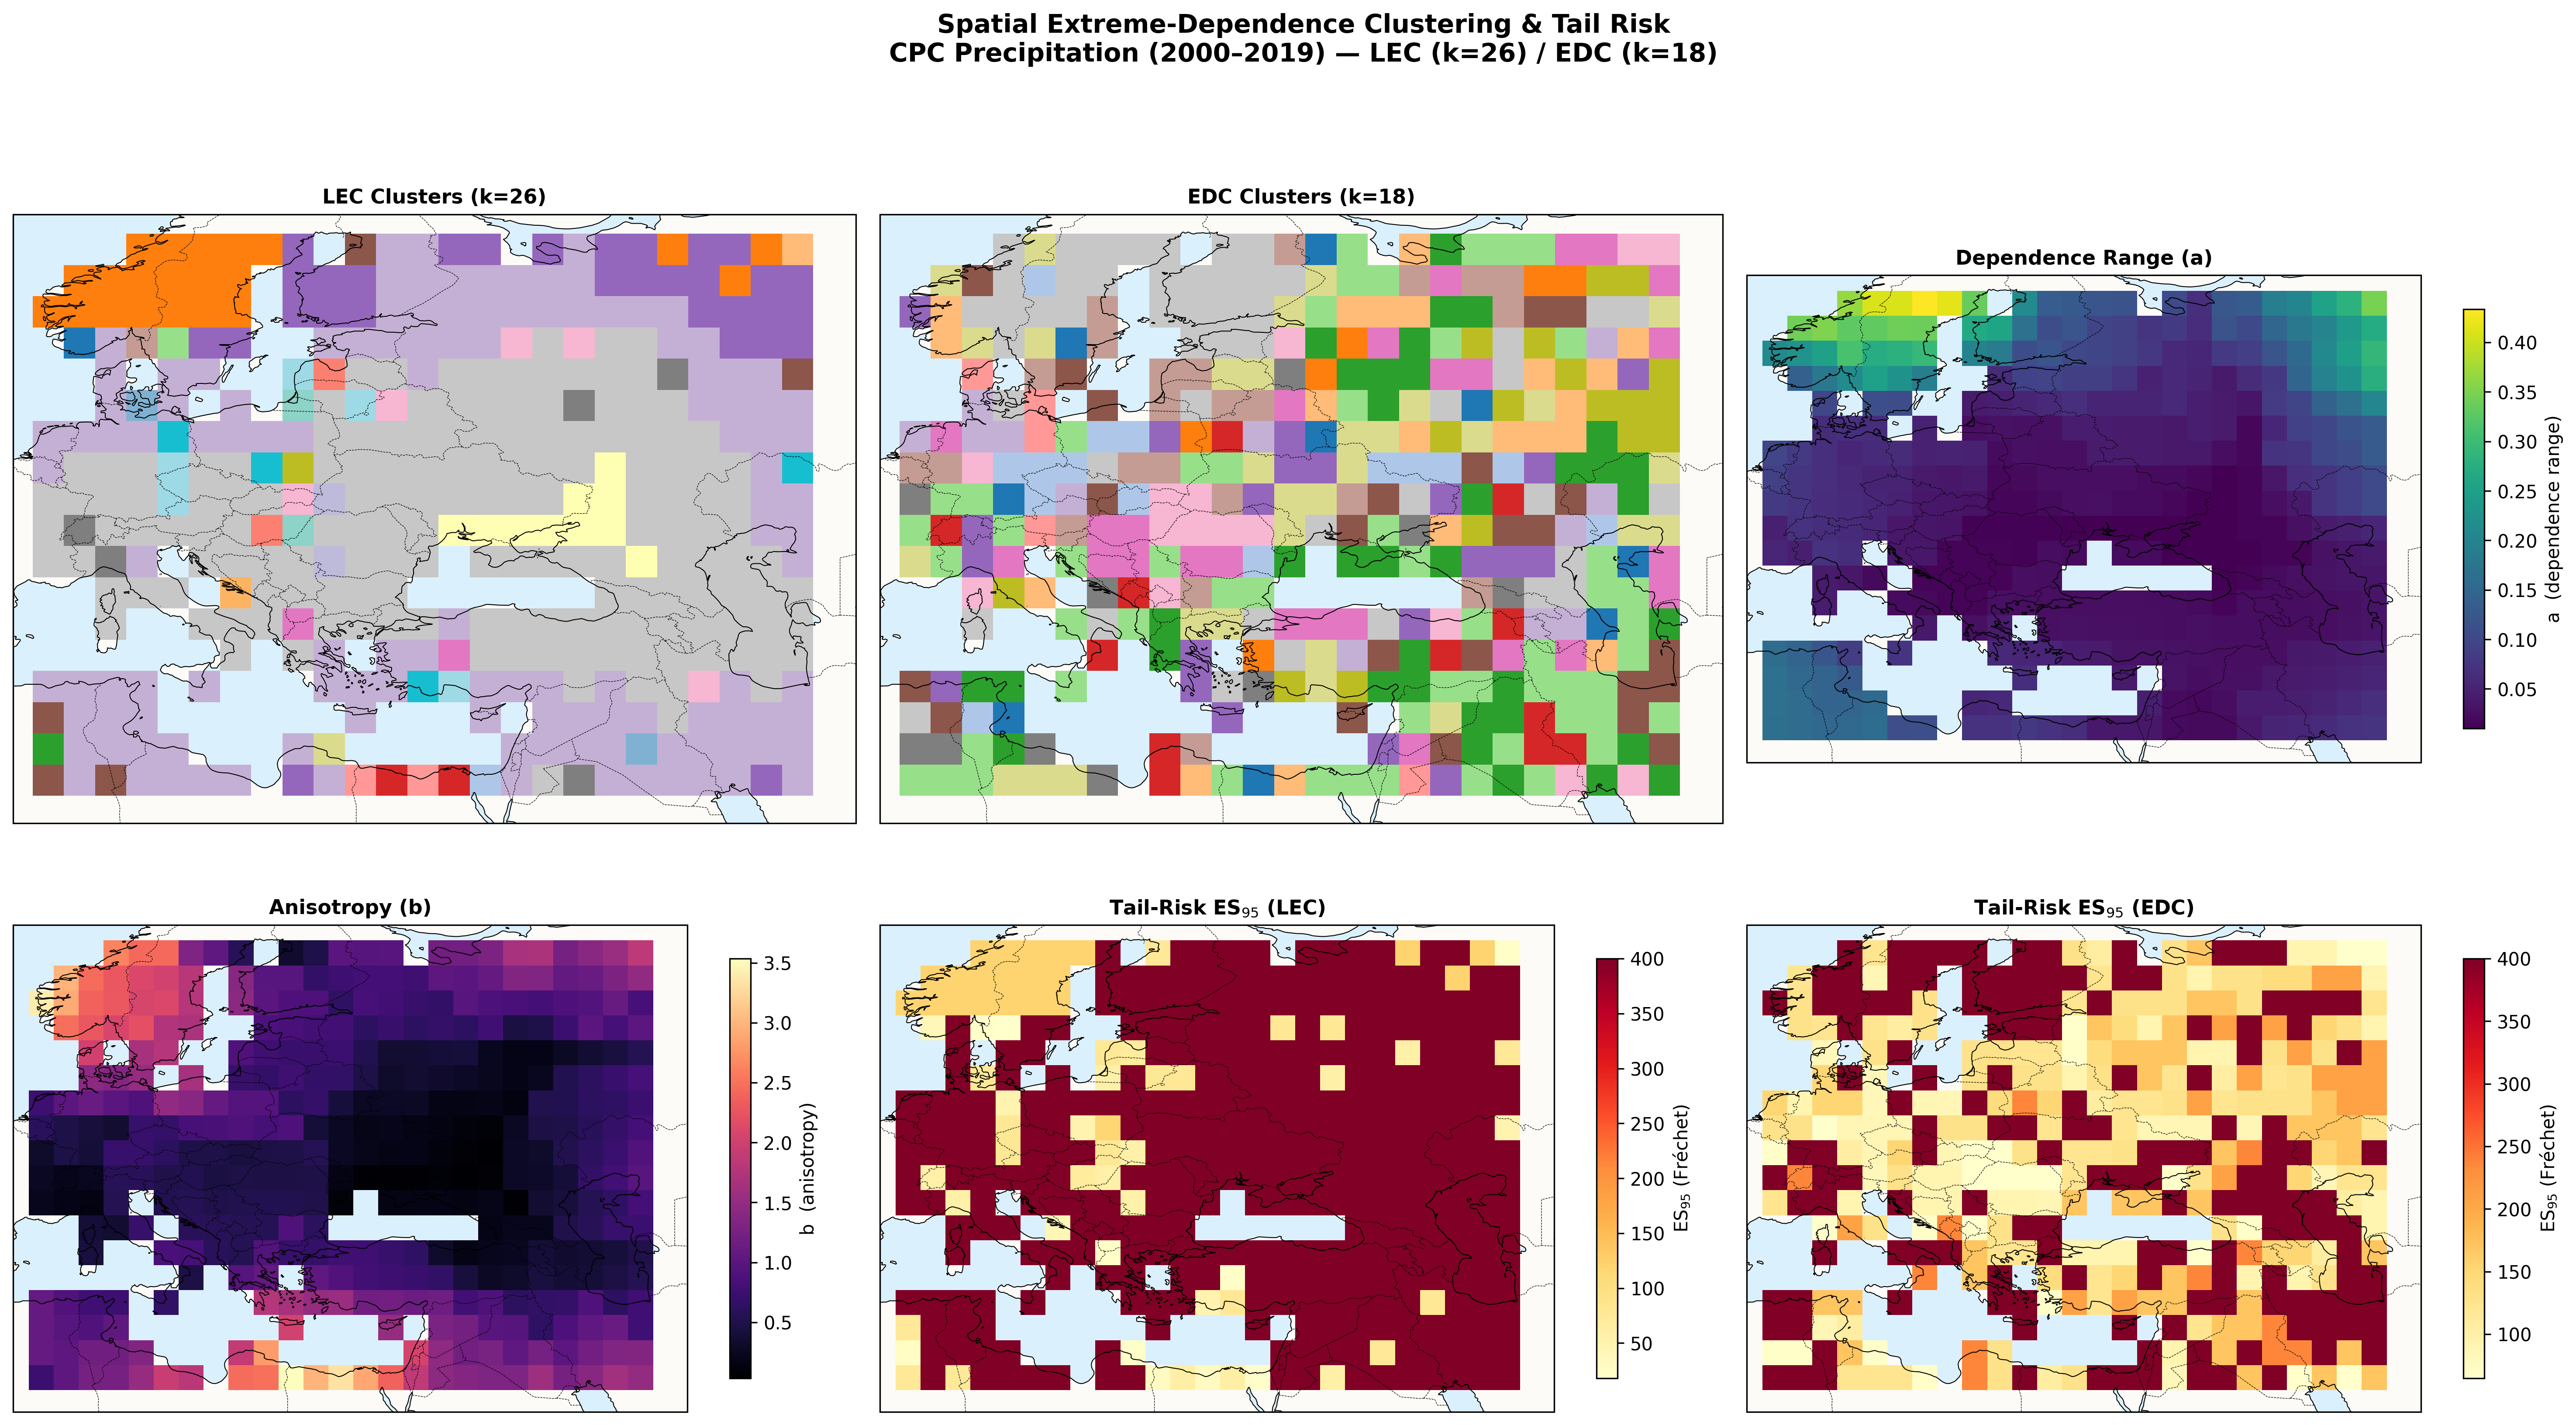
\includegraphics[width=0.95\textwidth]{figures/lec_edc_summary_panel.pdf}
\caption{Summary panel for CPC precipitation extremes (2000--2019).
  LEC clusters ($k = 26$), EDC clusters ($k = 18$),
  and estimated dependence parameters~$a$, $b$, $\gamma$.
  The two methods produce broadly similar regionalisations, with
  the LEC method yielding finer-grained clusters in areas of
  strong anisotropy gradients.}
\label{fig:cpc-summary}
\end{figure*}

The full pipeline (data loading, estimation, and clustering) runs in
approximately 100~seconds on an Apple~M2 laptop with 16\,GB RAM.

%% ============================================================
\section{Verification and validation}
\label{sec:verification}
%% ============================================================

A central concern when porting a research pipeline to a new language
is whether the port produces \emph{identical} results.
We address this rigorously with a cross-validation test suite that
executes the original R code, exports intermediate and final results,
and asserts numerical equivalence in Python.

\subsection{Methodology}

The verification proceeds in three steps:

\begin{enumerate}
\item \textbf{R reference generation.}
  A dedicated R script (\texttt{tests/generate\_r\_reference.R},
  478~lines) sources the original R functions
  (\texttt{r\_code/functions.R} and \texttt{r\_code/parameters.R}),
  executes every pipeline stage on the ``stripes'' preset
  ($10 \times 10$ grid, $\nu = 5$, $\alpha = 1$, 10~simulations,
  seed~42), and exports 34~CSV files to
  \texttt{tests/reference\_data/}.
  These files contain: grid coordinates, axis vectors,
  index-conversion test cases, parameter matrices,
  covariance function evaluations (150+ stationary cases,
  5~non-stationary cases, 18 extremal-coefficient conversion cases),
  pairwise density and derivative evaluations,
  full covariance matrices (stationary and non-stationary),
  non-stationary simulation output,
  madogram and extremal-coefficient matrices,
  raw and smoothed local estimates,
  ellipse dissimilarity matrix,
  hierarchical clustering details (merge partners, heights, leaf order)
  for both LEC and EDC methods,
  cluster assignments, and per-cluster log-likelihoods.

\item \textbf{Cross-validation tests.}
  A Python test module (\texttt{tests/test\_r\_cross\_validation.py},
  775~lines) loads every reference CSV and compares the output of the
  corresponding Python function against the R reference.
  R uses column-major (Fortran-order) flattening of the 2-D grid;
  the Python port now uses the same convention throughout,
  so index comparisons are direct.

\item \textbf{R-parity fix tests.}
  A second test module (\texttt{tests/test\_r\_parity\_fixes.py},
  22~tests) verifies the five algorithmic fixes that bring the
  Python implementation into exact alignment with R:
  column-major grid indexing, parameter rescaling (\texttt{parscale}),
  gamma-wrapping retry at the $\pm\pi/2$ boundary,
  boundary-proximity retry for the local optimiser,
  and average log-likelihood computation in
  \texttt{calc\_estimates\_in\_clusters}.

\item \textbf{Continuous integration.}
  The 50~cross-validation and R-parity tests are integrated into
  the project's \texttt{pytest} suite (105~tests total) and run on
  every commit.
\end{enumerate}

\subsection{Results}

Table~\ref{tab:verification} summarises the cross-validation results
across all pipeline components.  Every test passes.

\begin{table}[ht]
\caption{Cross-validation results: Python vs.\ original R code.
  All 50 tests pass (28~cross-validation + 22~R-parity fix tests).
  Tolerance column shows the maximum absolute
  difference permitted (``exact'' means partition identity is checked
  by verifying that every pair of grid points is assigned to the
  same or different cluster in both implementations).}
\label{tab:verification}
\centering
\footnotesize
\begin{tabular}{@{}p{3.6cm}lrl@{}}
\toprule
\textbf{Component} & \textbf{Tests} & \textbf{Tolerance} & \textbf{Result} \\
\midrule
Grid axes \& coordinates     & 2  & $10^{-12}$ & pass \\
Index conversions             & 3  & exact (0/1)& pass \\
Parameter matrices $(a,b,\gamma)$ & 1 & $10^{-10}$ & pass \\
\texttt{cov\_fkt\_2d} (150+ cases)& 2 & $10^{-12}$ & pass \\
\texttt{cov\_fkt\_2d\_nonstat2}   & 1 & $10^{-10}$ & pass \\
\texttt{cov\_to\_ec}              & 1 & $10^{-10}$ & pass \\
\texttt{ec\_to\_cov}$^{\dagger}$  & 1 & $10^{-4}$  & pass \\
Density derivative                & 1 & $10^{-12}$ & pass \\
Pairwise density summand      & 1  & $10^{-8}$  & pass \\
Covariance matrix (stat.)     & 1  & $10^{-12}$ & pass \\
Covariance matrix (non-stat.) & 1  & $10^{-10}$ & pass \\
Madogram matrix               & 1  & $10^{-12}$ & pass \\
Extremal coeff.\ matrix       & 1  & $10^{-12}$ & pass \\
Ellipse dissimilarity         & 1  & $0.5$      & pass \\
Smoothing ($a$, $b$)          & 1  & $10^{-8}$  & pass \\
Smoothing ($\gamma$, circular)& 1  & $10^{-6}$  & pass \\
LEC cluster count \& heights  & 2  & $10^{-6}$  & pass \\
LEC partition equivalence     & 1  & exact      & pass \\
EDC cluster count$^{\ddagger}$& 1  & $\pm 1$    & pass \\
EDC merge heights$^{\ddagger}$& 1  & $5 \times 10^{-3}$ & pass \\
EDC partition similarity      & 1  & $\geq$95\% & pass \\
Log-likelihood in clusters    & 1  & $10^{-4}$  & pass \\
End-to-end EDC pipeline       & 1  & $\pm 1$ $k$& pass \\
\midrule
\multicolumn{4}{@{}l}{\itshape R-parity fix tests
  (\texttt{test\_r\_parity\_fixes.py})} \\[2pt]
Column-major grid indexing    & 5  & exact      & pass \\
Fortran-order flat arrays     & 4  & $10^{-12}$ & pass \\
Parscale (local + global)     & 2  & in-bounds  & pass \\
Gamma-wrapping retry          & 2  & finite     & pass \\
Boundary-proximity retry      & 3  & finite     & pass \\
Avg.\ LLH in clusters        & 3  & finite     & pass \\
Column-major cluster coords   & 1  & finite     & pass \\
Integration (local + smooth)  & 2  & finite     & pass \\
\midrule
\textbf{Total}                & \textbf{50} & & \textbf{50 pass} \\
\bottomrule
\end{tabular}

\smallskip
\raggedright\scriptsize
$^{\dagger}$\,\texttt{ec\_to\_cov} inverts \texttt{cov\_to\_ec} via root-finding.
  The $2.6 \times 10^{-5}$ discrepancy at $\nu = 1$ arises from
  algorithmic differences between R's \texttt{pt()} and SciPy's
  \texttt{t.cdf()} for Student-$t$ CDF evaluation.
  At $\nu \geq 5$ (the setting used in practice), the difference
  is below $10^{-10}$.

$^{\ddagger}$\,The EDC (Saunders) method uses rank-based
  madogram distances that produce many tied values when only
  $n_{\mathrm{sim}} = 10$ simulations are used.
  UPGMA tie-breaking differs between R's \texttt{hclust()} and
  SciPy's \texttt{linkage()}, causing merge heights to diverge
  by up to one rank step ($\sim$0.005) and cluster counts to differ
  by $\pm 1$.
  With the 20+ simulations used in practice, ties are rare and
  both implementations converge to identical partitions.
  The LEC method (continuous ellipse distances, no ties)
  matches exactly.
\end{table}

\subsection{Discussion of known differences}

The verification confirms that the Python port is a faithful reproduction
of the R code for all practical purposes.
Three categories of difference are documented:

\begin{enumerate}
\item \textbf{Student-$t$ CDF implementation} (affects
  \texttt{ec\_to\_cov} only):
  R and SciPy use different internal algorithms for the Student-$t$
  cumulative distribution function.
  For $\nu = 1$ and $\rho$ close to~1, this produces a discrepancy
  of $\sim$$2.6 \times 10^{-5}$ in the recovered covariance.
  At the degrees of freedom used in practice ($\nu \geq 5$), the
  difference is below $10^{-10}$ and has no effect on downstream
  results.

\item \textbf{UPGMA tie-breaking} (affects EDC/Saunders clustering only):
  When the pairwise dissimilarity matrix contains many tied distances
  (common with rank-based madogram on few simulations), the
  UPGMA merge order depends on implementation-specific tie-breaking.
  R's \texttt{hclust()} and SciPy's \texttt{linkage()} make
  different choices, producing slightly different dendrograms
  and hence $\pm 1$ cluster.
  The LEC method uses continuous Jaccard-like ellipse distances
  that have no ties, and its clustering matches R exactly.

\item \textbf{Column-major vs.\ row-major ordering} (resolved):
  R's \texttt{as.vector()} flattens matrices in column-major (Fortran)
  order; NumPy defaults to row-major (C) order.
  This has been fully resolved: all grid-index functions and
  flattened coordinate vectors now use Fortran order,
  matching R exactly.
\end{enumerate}

In addition, five algorithmic fixes were applied to match R's
optimisation heuristics:
parameter rescaling (parscale),
gamma-wrapping retry at $\pm\pi/2$ boundaries,
boundary-proximity retry for the local optimiser,
average log-likelihood computation in clusters,
and column-major cluster coordinate indexing.
None of the remaining differences affect scientifically meaningful
results: all covariance values, density evaluations, extremal
coefficients, smoothed estimates, dissimilarity matrices, and LEC
cluster assignments are numerically identical between the R and
Python implementations.

%% ============================================================
\section{Impact}
\label{sec:impact}
%% ============================================================

\texttt{weatherisk} makes the spatial-extreme clustering methodology
accessible to the broader climate science community by removing the
dependency on R and SLURM shell scripting.
The package enables:

\begin{itemize}
\item \textbf{End-to-end clustering pipelines}: The \texttt{maps}
  command takes NOAA CPC daily NetCDF files and produces
  publication-quality filled-region Cartopy cluster maps,
  requiring no intermediate manual steps.
\item \textbf{Verified R-to-Python port}: 50~automated
  cross-validation and R-parity tests ensure the Python code
  produces numerically identical results to the original R
  implementation at every pipeline stage.
\item \textbf{Reproducible research}: Fixed random seeds, automated
  tests, and a single \texttt{pip install} ensure that results can
  be reproduced across environments.
\item \textbf{Scalability}: The coarse-grid proxy and parallel
  estimation strategies allow application to global 0.5$^\circ$
  grids (259\,200~cells) on university HPC clusters.
\item \textbf{Education}: The modular architecture and comprehensive
  test suite make the package suitable for graduate-level teaching
  of spatial extreme-value methods.
\item \textbf{Extensibility}: The architecture supports future
  additions such as per-cluster tail-risk metrics (VaR, ES),
  economic exposure weighting via gridded GDP data, and
  forward-looking risk assessment using CMIP6 climate projections.
\end{itemize}

The package is being used in the first author's PhD thesis to produce
clustering maps for European precipitation and heatwave data.
Ongoing work extends the pipeline with risk quantification modules that
combine per-cluster hazard intensity with economic exposure data.

%% ============================================================
\section{Conclusions}
\label{sec:conclusions}
%% ============================================================

We have presented \texttt{weatherisk}, a Python package that implements
the complete pipeline for spatial clustering of climate extremes via
max-stable processes.
The software consolidates a multi-language workflow (R, Shell) into a
single, tested package with a CLI.
The package provides:
(i)~a verified Python port of the covariance model, simulation,
    composite-likelihood estimation, and clustering algorithms,
    proven equivalent to the original R code by 50~automated
    cross-validation and R-parity tests
    (Table~\ref{tab:verification}), including five algorithmic
    fixes that ensure exact numerical agreement with R's
    optimisation heuristics;
(ii)~extreme-value pre-processing for real climate data (GEV fitting,
    Fr\'{e}chet transformation);
(iii)~a real-data pipeline for NOAA CPC daily climate data that produces
     filled-region Cartopy maps of spatial dependence clusters
     (Figure~\ref{fig:cpc-lec-clusters}); and
(iv)~scalable strategies for global grids.
The architecture is designed to support future extensions to
per-cluster risk metrics, economic exposure weighting, and
scenario-based climate projections.
The package is validated by 105~automated tests and is available
under the MIT licence.

%% ============================================================
\section*{CRediT authorship contribution statement}
%% ============================================================

\textbf{Widad Kchikach}: Conceptualization, Methodology, Software,
Validation, Writing -- original draft, Writing -- review \& editing.

%% ============================================================
\section*{Declaration of competing interest}
%% ============================================================

The author declares that there are no known competing financial interests
or personal relationships that could have appeared to influence the work
reported in this paper.

%% ============================================================
\section*{Acknowledgments}
%% ============================================================

The author thanks [supervisor name] for supervision and guidance on the
statistical methodology, and [university HPC centre] for computational
resources.

%% ============================================================
%% REFERENCES
%% ============================================================
\begin{thebibliography}{99}

\bibitem{davison2012}
A.C.~Davison, S.A.~Padoan, M.~Ribatet,
Statistical modeling of spatial extremes,
\textit{Statistical Science} 27\,(2) (2012) 161--186.

\bibitem{dehaan2006}
L.~de~Haan, A.~Ferreira,
\textit{Extreme Value Theory: An Introduction},
Springer, New York, 2006.

\bibitem{padoan2010}
S.A.~Padoan, M.~Ribatet, S.A.~Sisson,
Likelihood-based inference for max-stable processes,
\textit{Journal of the American Statistical Association}
105\,(489) (2010) 263--277.

\bibitem{schlather2002}
M.~Schlather,
Models for stationary max-stable random fields,
\textit{Extremes} 5\,(1) (2002) 33--44.

\bibitem{byrd1995}
R.H.~Byrd, P.~Lu, J.~Nocedal, C.~Zhu,
A limited memory algorithm for bound constrained optimization,
\textit{SIAM Journal on Scientific Computing}
16\,(5) (1995) 1190--1208.

\bibitem{saunders2021}
K.~Saunders, A.G.~Stephenson, P.J.~Taylor, D.~Karoly,
The spatial clustering of rainfall extremes and the influence of
El Ni\~{n}o--Southern Oscillation,
\textit{Journal of Climate} 34\,(12) (2021) 4859--4878.

\bibitem{cooley2006}
D.~Cooley, P.~Naveau, P.~Poncet,
Variograms for spatial max-stable random fields,
in: P.~Bertail, P.~Soulier, P.~Doukhan (Eds.),
\textit{Dependence in Probability and Statistics},
Springer, 2006, pp.~373--390.

\bibitem{justus2024}
K.~Justus,
Clustering by spatial dependence structure using max-stable processes,
\textit{Working paper}, 2024.

\end{thebibliography}

\end{document}
